\chapter{Implementarea}

În acest capitol va fi prezentata implementarea bibliotecii software pentru dezvoltarea de algoritmi și aplicații de recunoaștere a obiectelor.

Biblioteca a fost implementata într-un mod hibrid.
Interfețele au fost definite în limbajul C++, iar implementările au fost făcute atât în C++ cat și în Python.

Structura de directoare a bibliotecii este:
\verbatiminput{treeview.txt}
Fiecare pachet este situat in propriul director.
Declaratiile se gasesc in directorul "\verb!include!"
,iar implementarile in "\verb!src!".

\pagebreak
\section{Diagrama de clase}

\subsection{Core}
Pachetul "core" conține interfețe de baza ale bibliotecii.
\begin{figure}[H]
	\centering
		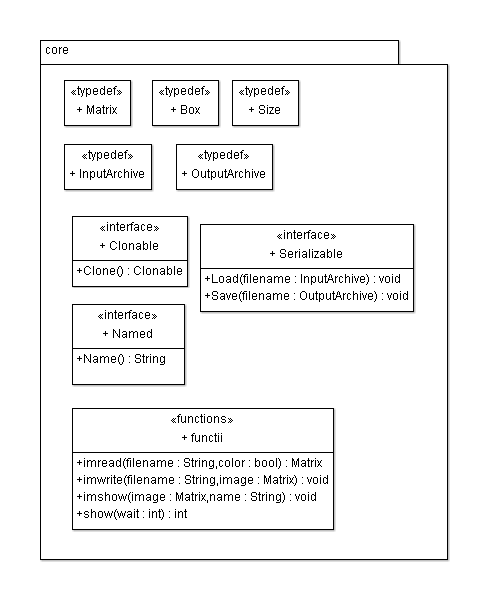
\includegraphics[width=0.95\textwidth]{uml/coreClassDiagram.png}
	\caption{core Class Diagram}
	\label{fig:coreClassDiagram}
\end{figure}

\subsection{Dataset}
Pachetul "dataset" conține clase care modelează baza de date pentru antrenament și implementează funcționalități de importare unor formate uzuale.
\begin{figure}[H]
	\centering
	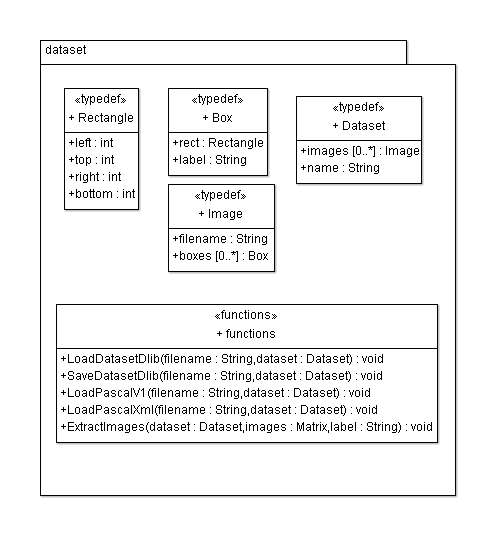
\includegraphics[width=1.0\textwidth]{uml/datasetClassDiagram.png}
	\caption{Diagrama de clase: dataset}
	\label{fig:datasetClassDiagram}
\end{figure}

\subsection{Image Pyramid}
Pachetul "image-pyramid" conține interfețe și implementări care servesc la construcția piramidei de imagini.
\begin{figure}[H]
	\centering
	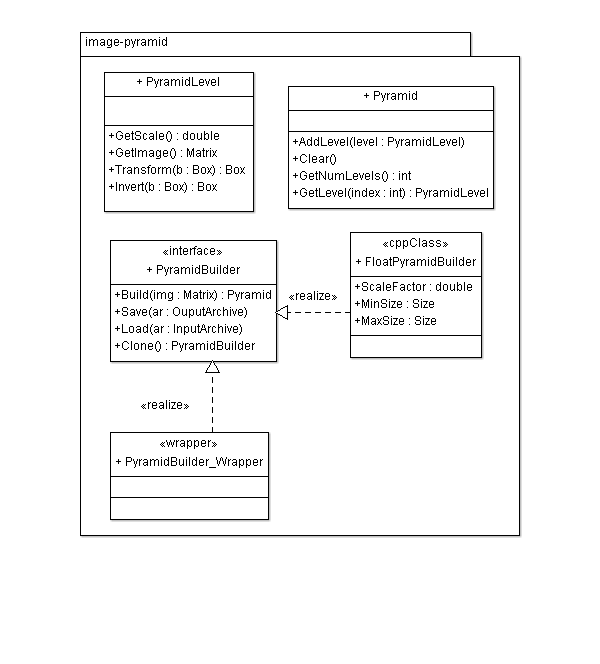
\includegraphics[width=1.00\textwidth]{uml/imagepyramidClassDiagram.png}
	\caption{Diagrama de clase: image-pyramid}
	\label{fig:imagepyramidClassDiagram}
\end{figure}


Clasa FloatPyramidBuilder construiește o piramida de imagini folosind ScaleFactor ca factor de scalare și MinSize, MaxSize ca criterii de terminare.

Metodele Transform si Invert din clasa PyramidLevel transforma coordonate din spațiul imaginii sursa în cel al nivelului, respectiv invers.

\subsection{Image Scanning}
Pachetul "image-scanning" conține interfețe și implementări care servesc la scanarea imaginilor
\begin{figure}[H]
	\centering
		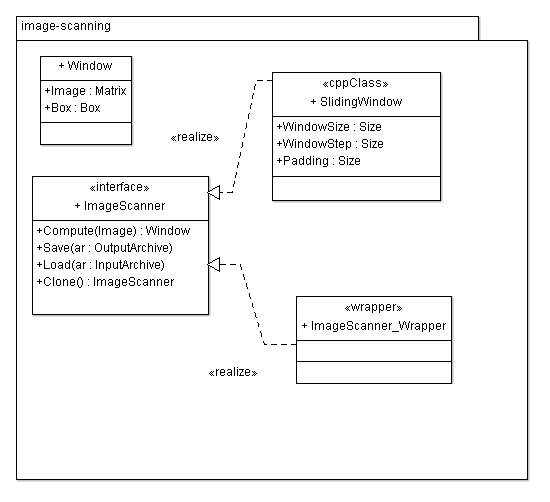
\includegraphics[width=1.00\textwidth]{uml/imagescanningClassDiagram.png}
	\caption{Diagrama de clase: image-scanning}
	\label{fig:imagescanningClassDiagram}
\end{figure}

\pagebreak
\subsection{Feature Extraction}
Pachetul "feature-extraction" conține interfețe și implementări care servesc la extragerea de trăsături din imagini.
\begin{figure}[H]
	\centering
		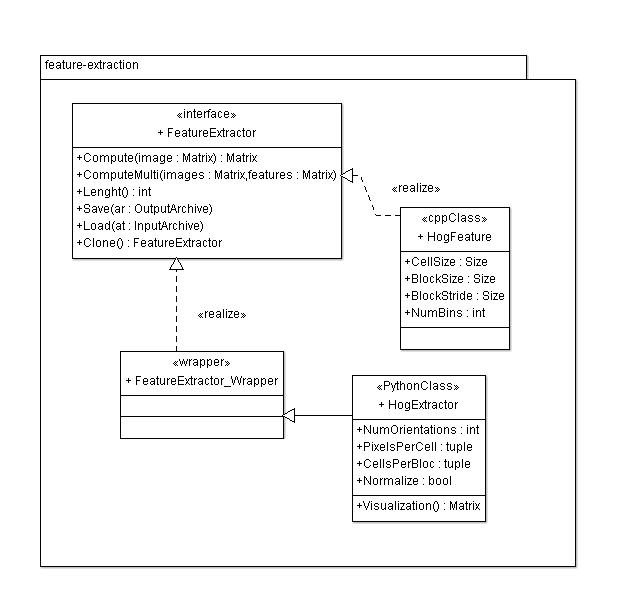
\includegraphics[width=1.00\textwidth]{uml/featureextractionClassDiagram.png}
	\caption{Diagrama de clase: feature-extraction}
	\label{fig:featureextractionClassDiagram}
\end{figure}

\pagebreak
\subsection{Classification}
Pachetul "classification" conține interfețe și implementări care servesc la clasificare și antrenarea clasificatorilor.
\begin{figure}[H]
	\centering
	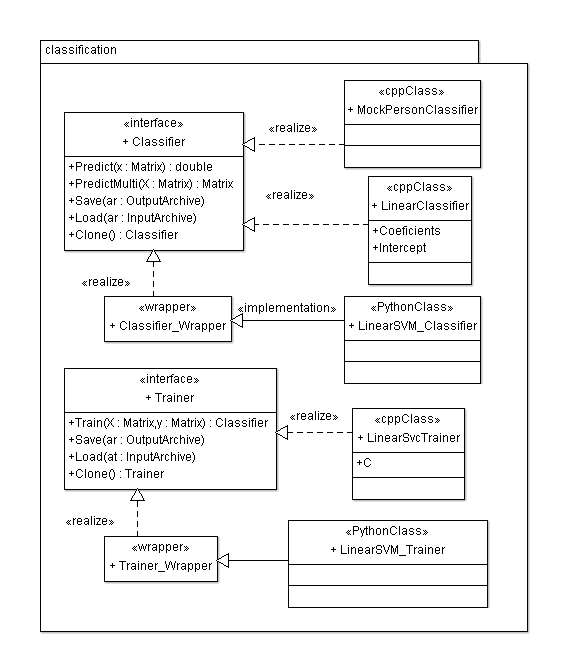
\includegraphics[width=1.00\textwidth]{uml/classificationClassDiagram.png}
	\caption{Diagrama de clase: classification}
	\label{fig:classificationClassDiagram}
\end{figure}

\subsection{Non Maxima Suppression}
Pachetul "non-maxima-suppression" conține interfețe și implementări care servesc la post-procesarea rezultatelor.
\begin{figure}[h]
	\centering
		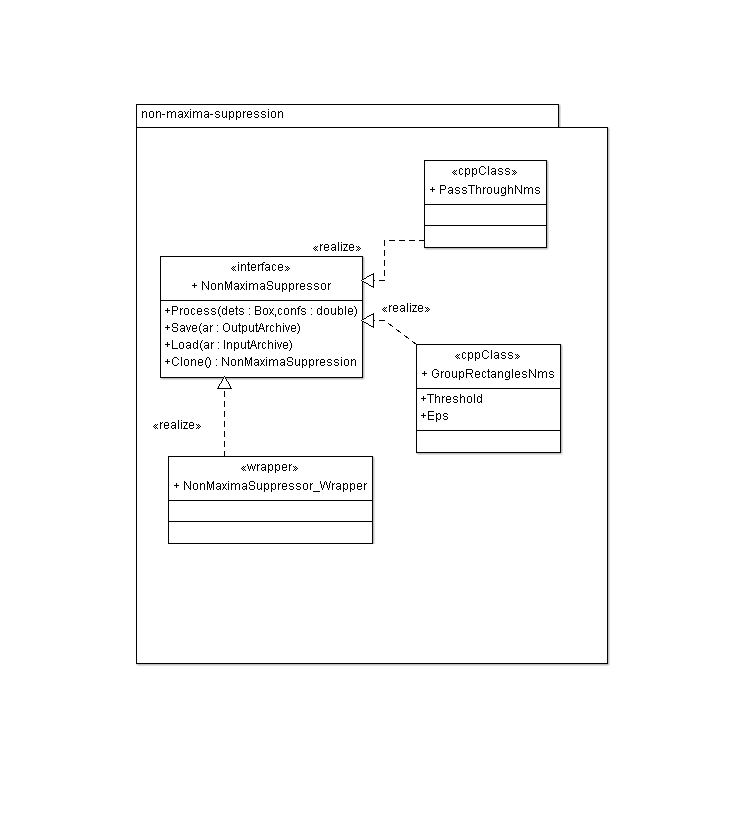
\includegraphics[width=1.00\textwidth]{uml/nonmaximasuppressionClassDiagram.png}
	\caption{Diagrama de clase: non-maxima-suppression}
	\label{fig:nonmaximasuppressionClassDiagram}
\end{figure}

\subsection{Detection}
Pachetul "detection" conține interfețe și implementări care servesc la recunoasterea obiectelor in imagini si la antrenarea algoritmilor.
\begin{figure}[H]
	\centering
		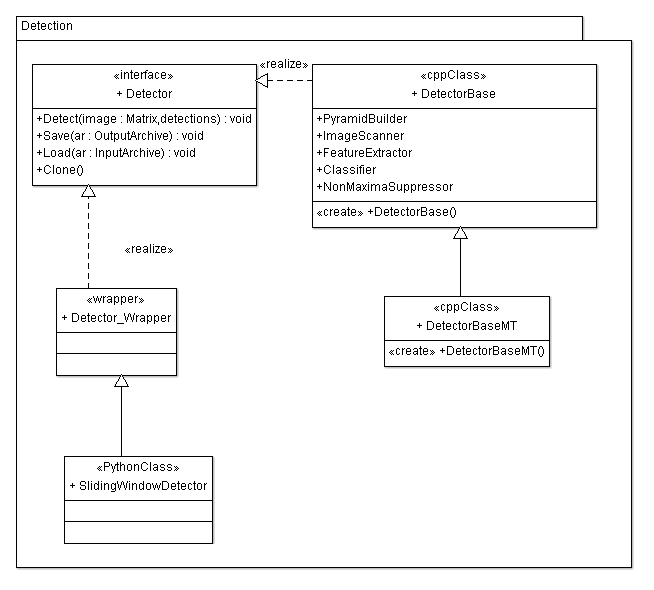
\includegraphics[width=1.00\textwidth]{uml/detectionClassDiagram.png}
	\caption{Diagrame de clase: detection}
	\label{fig:detectionClassDiagram}
\end{figure}
\begin{figure}[H]
	\centering
		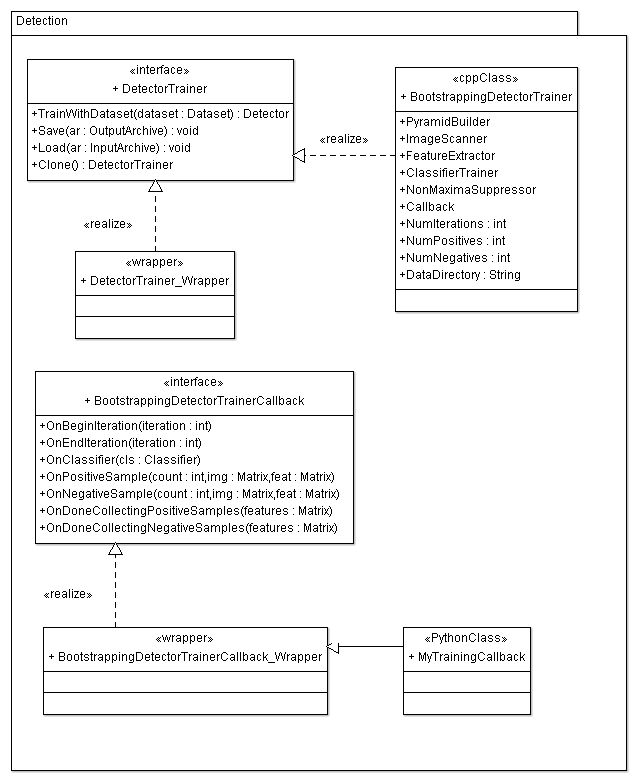
\includegraphics[width=1.00\textwidth]{uml/detection2ClassDiagram.png}
	\caption{Diagrama de clase: detection}
	\label{fig:detection2ClassDiagram}
\end{figure}

\pagebreak
\subsection{Python}
Pachetul "python" conține suportul necesar pentru interoperabilitatea cu limbajul Python.


\begin{figure}[H]
	\centering
		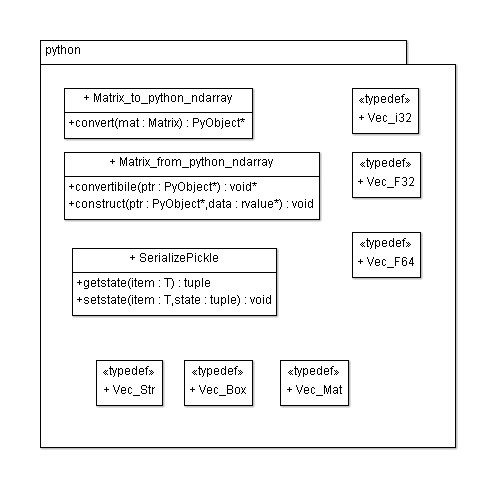
\includegraphics[width=1.00\textwidth]{uml/PythonClassDiagram.png}
	\caption{Diagrama de clase python}
	\label{fig:PythonClassDiagram}
\end{figure}




\pagebreak

\section{Interoperabilitatea cu Python}
\pagebreak

\section{Serializarea}
\pagebreak